\documentclass[conference]{IEEEtran}
\usepackage{amsmath,amssymb}
\usepackage{booktabs}
\usepackage{graphicx}
\usepackage[hidelinks]{hyperref}

\begin{document}

\title{Kernel Concentration and Bandwidth Scaling\\in Quantum Kernel Methods: Week~2 Progress}

\author{\IEEEauthorblockN{Muhammad Ahmad Masood and Muhammad Waqas}
\IEEEauthorblockA{AI 631 Quantum Machine Learning, Fall 2026 --- Project \#5}}

\maketitle

\begin{abstract}
We test, on three datasets, whether a bandwidth hyperparameter $\lambda$ keeps fidelity quantum kernels learnable as the qubit count grows. Following our proposal, an IQP kernel (all-to-all $ZZ$) and a Hamiltonian-evolution kernel are compared with a tuned RBF kernel on Fashion-MNIST images, AG News articles, and Speech Commands clips, reduced by PCA to 2--16 components, in exact and finite-shot simulation and under an IBM calibration noise model. At $\lambda=1$ the off-diagonal kernel variance falls exponentially with the qubit count on every dataset (slopes $-0.58$ to $-1.34$ per qubit). With a tuned $\lambda$ the kernel spread stays hundreds of times above the 5{,}000-shot noise floor, and test accuracy is far above chance. The quantum kernels match RBF on Fashion-MNIST, while on Speech Commands the IQP kernel is significantly worse than RBF, which triggers our falsifier for that kernel.
\end{abstract}

\section{Introduction}
Fidelity quantum kernels compare data points through the overlap of encoded states~\cite{havlicek2019supervised}. As the number of qubits grows, these overlaps can concentrate exponentially around a common value, so the kernel matrix approaches the identity and becomes impossible to estimate with a polynomial number of shots~\cite{thanasilp2024concentration,huang2021power}. Rescaling the inputs by a bandwidth $\lambda<1$ can restore generalization~\cite{shaydulin2022bandwidth}.

\textbf{Research question.} How fast do quantum kernel values concentrate as the qubit count grows, and does a bandwidth hyperparameter restore learnability?

\textbf{Hypotheses and falsifier} (from our proposal). \emph{H1:} at $\lambda=1$ the off-diagonal variance decays exponentially with the qubit count; it is rejected unless the 95\% interval of the slope of $\ln\mathrm{Var}(K_{ij})$ lies below zero. \emph{H2:} with a cross-validated $\lambda^{*}$, at $n=16$ and 5{,}000 shots, the kernel stays measurable and accurate; it is rejected if (a) $\mathrm{Var}(K_{ij})<\overline{K_{ij}(1-K_{ij})}/5000$, (b) accuracy is not above chance (one-sided binomial test), or (c) accuracy is significantly below the tuned RBF kernel (exact two-sided McNemar test, $\alpha=0.05$).

This stage implements the full proposal design and adds two datasets from other modalities, text and audio, to test whether the conclusions depend on the data.

\section{Methods}
\textbf{Data.} Each dataset is a balanced binary task with 1{,}200 training and 200 held-out test samples drawn from the official partitions (seeds 42 and 43). \emph{Fashion-MNIST}~\cite{xiao2017fashion}: T-shirt/top vs.\ Pullover, 784 pixels. \emph{AG News}~\cite{zhang2015character}: Business vs.\ Sci/Tech, 1{,}000-term TF-IDF vectors with the vocabulary fitted on 20{,}000 disjoint training articles. \emph{Speech Commands v0.02}~\cite{warden2018speech}: ``yes'' vs.\ ``no'', 800 log-mel features per one-second clip; the official split keeps speakers apart. Five fixed stratified folds (960/240) are used for model selection; a standardizer and 16-component PCA are fit on each fold's training rows, and the first $n\in\{2,4,\dots,16\}$ components form the sweep.

\textbf{Kernels.} The IQP map applies $U_Z(\lambda\mathbf{x})H^{\otimes n}U_Z(\lambda\mathbf{x})H^{\otimes n}$ with $U_Z(\mathbf{u})=\exp(i\sum_j u_jZ_j+i\sum_{j<k}u_ju_kZ_jZ_k)$ on $n$ qubits. The Hamiltonian map evolves a fixed Haar-random product state on $n+1$ qubits under nearest-neighbour Heisenberg bonds weighted by $\lambda x_j$, with $T=40$ Trotter steps. The kernel is $K_{ij}=|\langle\psi(\mathbf{x}_j)|\psi(\mathbf{x}_i)\rangle|^{2}$, computed from exact statevectors and checked against Qiskit circuits to within $10^{-13}$. At $n=16$ an IQP feature map has 240 two-qubit rotations (480 CX after compilation to all-to-all connectivity, depth 142); the 17-qubit Hamiltonian map has 1{,}920 (3{,}840 CX, depth 1{,}412). A kernel circuit applies the map and its inverse, doubling these counts.

\textbf{Selection, shots, and noise.} $\lambda\in\{10^{-3},10^{-2},10^{-1},1\}$ (RBF: $\gamma\in\{10^{-4},\dots,10^{-1}\}$) and 18 values of $C$ from 0.006 to 1{,}024 are chosen by five-fold accuracy, separately for exact and 5{,}000-shot kernels. Finite-shot entries are binomial draws for $N\in\{10^{2},10^{3},5{\times}10^{3},10^{4},10^{5}\}$, and noisy training matrices are projected onto the nearest PSD matrix. H1 uses all 719{,}400 training pairs with a 1{,}000-sample bootstrap. Noise uses Qiskit Aer with an archived IBM Manila calibration snapshot; physical-device runs are pending.

\begin{figure*}[t]
\centering
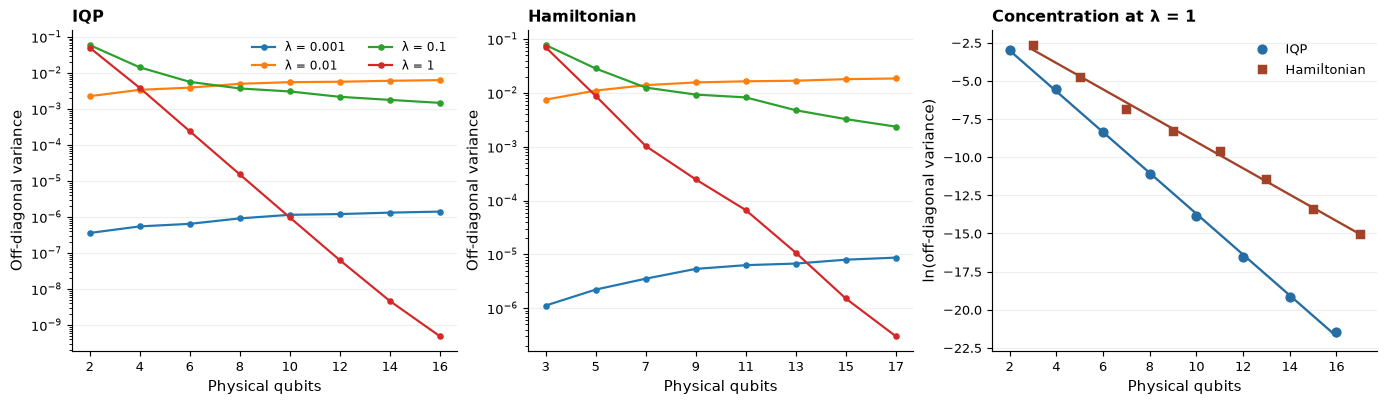
\includegraphics[width=\textwidth]{figures/concentration_fmnist.png}
\caption{Fashion-MNIST: exact off-diagonal kernel variance vs.\ physical qubits for each bandwidth, for the IQP (left) and Hamiltonian (middle) kernels, and the log-linear fit at $\lambda=1$ (right). AG News and Speech Commands show the same pattern (slopes in Table~\ref{tab:conc}).}
\label{fig:conc}
\end{figure*}

\section{Results}
\begin{table}[t]
\centering
\caption{Held-out accuracy (\%, 200 samples) at $n=16$ components (16 qubits IQP, 17 Hamiltonian). $p$: exact McNemar test of the 5{,}000-shot kernel vs.\ RBF.}
\label{tab:acc}
\setlength{\tabcolsep}{3pt}
\begin{tabular}{lccccccc}
\toprule
& \multicolumn{3}{c}{IQP} & \multicolumn{3}{c}{Hamiltonian} & RBF \\
Data & exact & 5k & $p$ & exact & 5k & $p$ & \\
\midrule
Fashion-MNIST & 95.0 & 94.5 & 0.25 & 94.5 & 95.5 & 1.00 & 96.0 \\
AG News & 77.0 & 79.5 & 0.049 & 76.0 & 74.5 & 1.00 & 75.0 \\
Speech Cmds & 95.5 & 92.5 & 0.008 & 94.0 & 94.5 & 0.22 & 96.5 \\
\bottomrule
\end{tabular}
\end{table}

\begin{table}[t]
\centering
\caption{Concentration at $\lambda=1$ (slope of $\ln\mathrm{Var}(K_{ij})$ per physical qubit, 95\% bootstrap interval) and spread at the 5{,}000-shot $\lambda^{*}$ relative to the single-entry shot-noise floor at $n=16$.}
\label{tab:conc}
\setlength{\tabcolsep}{3pt}
\begin{tabular}{lcccc}
\toprule
& \multicolumn{2}{c}{Slope at $\lambda=1$} & \multicolumn{2}{c}{Spread / floor at $\lambda^{*}$} \\
Data & IQP & Hamiltonian & IQP & Ham. \\
\midrule
Fashion-MNIST & $-1.34$ & $-0.86$ & 391 & 678 \\
AG News & $-0.70$ & $-0.76$ & 1{,}184 & 1{,}561 \\
Speech Cmds & $-0.58$ & $-0.63$ & 202 & 563 \\
\bottomrule
\end{tabular}
\end{table}

\textbf{Concentration (H1).} At $\lambda=1$ the variance falls exponentially on all three datasets (Fig.~\ref{fig:conc}); every 95\% interval lies below zero, from $[-1.341,-1.334]$ (Fashion-MNIST IQP) to $[-0.777,-0.494]$ (Speech IQP). At $n=16$ and $\lambda=1$ the Fashion-MNIST IQP variance is $4.9\times10^{-10}$. H1 is not rejected.

\textbf{Measurability (H2a, b).} The selected bandwidth is small ($\lambda^{*}=0.01$, or 0.1 on AG News), and the spread there exceeds the 5{,}000-shot floor by a factor of 202 to 1{,}561 (Table~\ref{tab:conc}); 4 to 25 shots would already bring the noise below the spread. All kernels are far above chance (binomial $p\le1.3\times10^{-12}$). A tuned $\lambda$ also beats $\lambda=1$ in the 20-seed Hamiltonian control at $n=4$: 94.0\% vs.\ 81.8\% (Fashion-MNIST), 79.2\% vs.\ 67.4\% (AG News), and 81.0\% vs.\ 63.5\% (Speech).

\textbf{Comparison with RBF (H2c).} On Fashion-MNIST neither kernel differs significantly from RBF. On AG News the IQP kernel is better than RBF (13 vs.\ 4 discordant samples, $p=0.049$). On Speech Commands the IQP kernel is significantly worse (0 vs.\ 8, $p=0.008$), so \emph{H2 is rejected for the IQP kernel on Speech Commands}; the Hamiltonian kernel passes every criterion on all three datasets.

\textbf{Shots and noise.} At $n=16$ accuracy rises with the shot count, e.g.\ the Speech IQP kernel from 79.5\% at $10^{2}$ shots to 94.5\% at $10^{5}$. In the Manila noise model, the self-overlap $K_{ii}$ drops from 1 to about 0.89 (IQP, 2 qubits), 0.42--0.44 (IQP, 4 qubits), and 0.15 (Hamiltonian, 3 qubits, 960 two-qubit gates). The noisy 2-qubit IQP classifier reaches 92.5--93.5\% on Fashion-MNIST but only 57.5--64.5\% on AG News and Speech Commands.

\section{Discussion}
Concentration at $\lambda=1$ is exponential for both feature maps and all three modalities, and a small bandwidth keeps the kernel both informative and measurable at 5{,}000 shots. Bandwidth does not give a consistent advantage over RBF: the two significant differences go in opposite directions, and each comes from a single 200-sample test set, so neither should be read as a general effect; with several comparisons, one $p$-value near 0.05 is expected by chance. The coarse four-value $\lambda$ grid is a limitation, since the exact Fashion-MNIST winners sit at its lowest value. The noise model shows that deep circuits, especially the Hamiltonian map, lose most of their signal on current devices. Next steps are a finer $\lambda$ grid, repeated splits, and physical IBM runs at 2--3 qubit counts.

\textbf{Reproducibility.} All three notebooks were re-executed end to end (Python 3.12, Qiskit 2.6.2, Aer 0.17.2, scikit-learn 1.8.0). The Fashion-MNIST rerun reproduced every saved result table. Two environment notes: Qiskit circuit drawing needs \texttt{pylatexenc}, and with pandas~3 the OpenML loader fails, so the Fashion-MNIST sample was rebuilt from the official files with checksum verification.

\bibliographystyle{IEEEtran}
\bibliography{refs}

\end{document}
